\documentclass[handout]{ximera}

%% You can put user macros here
%% However, you cannot make new environments



\newcommand{\ffrac}[2]{\frac{\text{\footnotesize $#1$}}{\text{\footnotesize $#2$}}}
\newcommand{\vasymptote}[2][]{
    \draw [densely dashed,#1] ({rel axis cs:0,0} -| {axis cs:#2,0}) -- ({rel axis cs:0,1} -| {axis cs:#2,0});
}


\graphicspath{{./}{firstExample/}}

\usepackage{amsmath}
\usepackage{amssymb}
\usepackage{array}
\usepackage[makeroom]{cancel} %% for strike outs
\usepackage{pgffor} %% required for integral for loops
\usepackage{tikz}
\usepackage{tikz-cd}
\usepackage{tkz-euclide}
\usetikzlibrary{shapes.multipart}


\usetkzobj{all}
\tikzstyle geometryDiagrams=[ultra thick,color=blue!50!black]


\usetikzlibrary{arrows}
\tikzset{>=stealth,commutative diagrams/.cd,
  arrow style=tikz,diagrams={>=stealth}} %% cool arrow head
\tikzset{shorten <>/.style={ shorten >=#1, shorten <=#1 } } %% allows shorter vectors

\usetikzlibrary{backgrounds} %% for boxes around graphs
\usetikzlibrary{shapes,positioning}  %% Clouds and stars
\usetikzlibrary{matrix} %% for matrix
\usepgfplotslibrary{polar} %% for polar plots
\usepgfplotslibrary{fillbetween} %% to shade area between curves in TikZ



%\usepackage[width=4.375in, height=7.0in, top=1.0in, papersize={5.5in,8.5in}]{geometry}
%\usepackage[pdftex]{graphicx}
%\usepackage{tipa}
%\usepackage{txfonts}
%\usepackage{textcomp}
%\usepackage{amsthm}
%\usepackage{xy}
%\usepackage{fancyhdr}
%\usepackage{xcolor}
%\usepackage{mathtools} %% for pretty underbrace % Breaks Ximera
%\usepackage{multicol}



\newcommand{\RR}{\mathbb R}
\newcommand{\R}{\mathbb R}
\newcommand{\C}{\mathbb C}
\newcommand{\N}{\mathbb N}
\newcommand{\Z}{\mathbb Z}
\newcommand{\dis}{\displaystyle}
%\renewcommand{\d}{\,d\!}
\renewcommand{\d}{\mathop{}\!d}
\newcommand{\dd}[2][]{\frac{\d #1}{\d #2}}
\newcommand{\pp}[2][]{\frac{\partial #1}{\partial #2}}
\renewcommand{\l}{\ell}
\newcommand{\ddx}{\frac{d}{\d x}}

\newcommand{\zeroOverZero}{\ensuremath{\boldsymbol{\tfrac{0}{0}}}}
\newcommand{\inftyOverInfty}{\ensuremath{\boldsymbol{\tfrac{\infty}{\infty}}}}
\newcommand{\zeroOverInfty}{\ensuremath{\boldsymbol{\tfrac{0}{\infty}}}}
\newcommand{\zeroTimesInfty}{\ensuremath{\small\boldsymbol{0\cdot \infty}}}
\newcommand{\inftyMinusInfty}{\ensuremath{\small\boldsymbol{\infty - \infty}}}
\newcommand{\oneToInfty}{\ensuremath{\boldsymbol{1^\infty}}}
\newcommand{\zeroToZero}{\ensuremath{\boldsymbol{0^0}}}
\newcommand{\inftyToZero}{\ensuremath{\boldsymbol{\infty^0}}}


\newcommand{\numOverZero}{\ensuremath{\boldsymbol{\tfrac{\#}{0}}}}
\newcommand{\dfn}{\textbf}
%\newcommand{\unit}{\,\mathrm}
\newcommand{\unit}{\mathop{}\!\mathrm}
%\newcommand{\eval}[1]{\bigg[ #1 \bigg]}
\newcommand{\eval}[1]{ #1 \bigg|}
\newcommand{\seq}[1]{\left( #1 \right)}
\renewcommand{\epsilon}{\varepsilon}
\renewcommand{\iff}{\Leftrightarrow}

\DeclareMathOperator{\arccot}{arccot}
\DeclareMathOperator{\arcsec}{arcsec}
\DeclareMathOperator{\arccsc}{arccsc}
\DeclareMathOperator{\si}{Si}
\DeclareMathOperator{\proj}{proj}
\DeclareMathOperator{\scal}{scal}
\DeclareMathOperator{\cis}{cis}
\DeclareMathOperator{\Arg}{Arg}
%\DeclareMathOperator{\arg}{arg}
\DeclareMathOperator{\Rep}{Re}
\DeclareMathOperator{\Imp}{Im}
\DeclareMathOperator{\sech}{sech}
\DeclareMathOperator{\csch}{csch}
\DeclareMathOperator{\Log}{Log}

\newcommand{\tightoverset}[2]{% for arrow vec
  \mathop{#2}\limits^{\vbox to -.5ex{\kern-0.75ex\hbox{$#1$}\vss}}}
\newcommand{\arrowvec}{\overrightarrow}
\renewcommand{\vec}{\mathbf}
\newcommand{\veci}{{\boldsymbol{\hat{\imath}}}}
\newcommand{\vecj}{{\boldsymbol{\hat{\jmath}}}}
\newcommand{\veck}{{\boldsymbol{\hat{k}}}}
\newcommand{\vecl}{\boldsymbol{\l}}
\newcommand{\utan}{\vec{\hat{t}}}
\newcommand{\unormal}{\vec{\hat{n}}}
\newcommand{\ubinormal}{\vec{\hat{b}}}

\newcommand{\dotp}{\bullet}
\newcommand{\cross}{\boldsymbol\times}
\newcommand{\grad}{\boldsymbol\nabla}
\newcommand{\divergence}{\grad\dotp}
\newcommand{\curl}{\grad\cross}
%% Simple horiz vectors
\renewcommand{\vector}[1]{\left\langle #1\right\rangle}


\pgfplotsset{compat=1.13}

\outcome{Explore special sequences}

\title{3.1 Sequences}

\begin{document}

\begin{abstract}
We will explore special sequences.
\end{abstract}

\maketitle

\section{Sequences}
A sequence is a list of numbers. The length of the sequence can be either finite or infinite. For example,
the sequence of binomial coefficients,
\[
\binom{n}{0}, \binom{n}{1}, \binom{n}{2}, \dots, \binom{n}{n}
\]
is a sequence of length $n+1$ when $n\in \mathbb{N}$, whereas the sequence
\[
\binom{\alpha}{0}, \binom{\alpha}{1}, \binom{\alpha}{2} \dots, 
\]
has infinitely many terms for $\alpha \in \mathbb{R}$.
(Actually, if we recall from section 1.11, $\binom{n}{k}$ is defined to be $0$ for $k,n \in \mathbb{N}$ with $k > n$, 
so the first sequence can be extended indefinitely with infinitely many zero terms.)
We have also seen sequences defined recursively. Recall that for the derangement numbers $D_n$ we have
\[
D_n = (n-1)(D_{n-2} + D_{n-1})
\]
as long as we have values for $D_0$ and $D_1$ (seeds), we can find $D_2, D_3, D_4$ and so on.
We begin with some elementary sequences and then we will explore the important Fibonacci sequence.

\begin{example}[Example 1]
Let $a, d \in \mathbb{R}$ and define the sequence $\{a_n\}$ recursively by $a_0 = a$ and $a_n = a_{n-1} + d$.  (This is known as an arithmetic sequence.)
Find $a_1, a_2, a_3, a_4$ then conjecture a formula for $a_n$ and verify your conjecture using mathematical induction.\\
According to the recursive formula for $a_n$, we have
\begin{align*}
a_1 &= a_0 + d= a+d\\
a_2 &= a_1 + d= a+2d\\
a_3 &= a_2 + d= a+3d\\
a_4 &= a_3 + d= a+4d\\
\end{align*}
It is now clear that our conjecture is $a_n = a + nd$ and we prove this by induction. The base case for $n=1$ is true as indicated above.
We now suppose that $a_n = a + nd$ for some $n \in \mathbb{N}$ and we want to show that $a_{n+1} = a + (n+1)d$. 
By the recursive definition of the sequence we have,
\[
a_{n+1} = a_n + d
\]
and by the inductive hypothesis $a_n = a + nd$, so
\[
a_{n+1} = a + nd + d = a + (n+1)d
\]
as desired. By induction, $a_n = a + nd$ for all $n \in \mathbb{N}$.
\end{example}

\begin{problem}(problem 1a)
Let $a, r \in \mathbb{R}$ and define the sequence $\{a_n\}$ recursively by $a_0 = a$ and $a_n = ra_{n-1} $.  (This is known as a geometric sequence.)
Find $a_1, a_2, a_3, a_4$ then conjecture a formula for $a_n$ and verify your conjecture using mathematical induction.\\
\end{problem}

\begin{problem}(problem 1b)
Consider the sequence of partial sums of the geometric sequence from problem 1a. That is, let
\[
s_n = \sum_{k=0}^n a_k = a_0 + a_1 + \dots + a_n
\]
Use induction (with base case $n=1$) to prove that for $r \neq 1$
\[
s_n = a\left(\frac{1-r^{n+1}}{1-r}\right)
\]
\end{problem}

\begin{problem}(problem 1c)
Define the sequence $\{a_n\}$ recursively by $a_0 = 1$ and $a_n = na_{n-1} $.  
Find $a_1, a_2, a_3, a_4$ then conjecture a formula for $a_n$ and verify your conjecture using mathematical induction.\\
\end{problem}

\section{Fibonacci Sequence}
Consider the following population problem: a pair of baby rabbits (one male, one female) reach adulthood after one month. 
Assuming that each month a pair of adult rabbits will produce a pair of baby rabbits (one male, one female), 
how many pairs of rabbits will there be after $n$ months? During month $1$, we have one pair of baby rabbits which we will denote by 'r'.
During month $2$, we have one pair of adult rabbits, R. During month $3$, we have one pair of adult rabbits and one pair of baby rabbits, rR.
During month $4$, we have two pairs of adult rabbits and one pair of baby rabbits, rRR. And so on. 
If we know how many pairs of rabbits of each type we have during a particular month, 
then we can determine how may pairs of each type we will have during the next month and how many of each type we had during the previous month.
For example, if we now have $m$ pairs of baby rabbits and $n$ pairs of adult rabbits, 
then the next month we will have $m+n$ pairs of adult rabbits and $n$ pairs of baby rabbits, 
for a total of $m+2n$ pairs of rabbits.  
Furthermore, during the previous month we must have had $m$ pairs of adult rabbits and $n-m$ pairs of baby rabbits, 
for a total of $n$ pairs of rabbits.
From this we can see that the number of rabbits at a particular time is the sum of the number of pairs of rabbits from the previous 2 months.
This motivates the following definition of the Fibonacci sequence:

\begin{definition}[Fibonacci Sequence]
The Fibonacci sequence is defined recursively by letting $f_1 = f_2 = 1$ and then
\[
f_n = f_{n-2} + f_{n-1}\;\; \text{for}\;\; n \geq 3
\]
\end{definition}

The first 10 terms of the Fibonacci sequence are
\[
1, 1, 2, 3, 5, 8, 13, 21, 34, 55,...
\]
We now look at some interesting properties of the sequence which can be proven using induction.

\begin{example}[example 3]
Use induction to prove that for each $n \in \mathbb{N}, f_{3n}$ is even.\\
Base case: if $n=1$ then $f_{3n} = f_3 = f_1 + f_2 = 1+1 = 2$ which is even.\\
Inductive Hypothesis: Suppose that $f_{3n}$ is even for some $n \in \mathbb{N}$.\\
Inductive Step: We want to show that $f_{3(n+1)} = f_{3n+3}$ is even.\\
By the recursive definition of the Fibonacci sequence, we have 
\begin{align*}
f_{3n+3} &= f_{3n+1} + f_{3n+2}\\
        &= f_{3n+1} + f_{3n} + f_{3n+1}\\
        &= f_{3n} + 2f_{3n+1}\\
        &= \text{even} \; + \; \text{even}\\
        &= \text{even}
\end{align*}
Hence, $f_{3n}$ is even for all $n \in \mathbb{N}$.
\end{example} 

\begin{problem}(problem 3)
Use induction to prove that for all  $n \in \mathbb{N}$,
\[
f_1 + f_2 + \cdots + f_n = f_{n+2} - 1
\]
\end{problem}

Our next goal is to find a non-recursive formula for $f_n$. To this end, 
we will examine the ratios of the terms of the Fibonacci sequence. Since
\[
f_{n+2} = f_n + f_{n+1},
\]
we can divide by $f_{n+1}$ to obtain
\[
\frac{f_{n+2}}{f_{n+1}} = \frac{f_{n}}{f_{n+1}} + 1
\]
Taking the limit gives
\[
\lim_{n \to \infty} \frac{f_{n+2}}{f_{n+1}} = \lim_{n \to \infty} \frac{f_{n}}{f_{n+1}} + 1
\]
Assuming the limit on the left-hand side exists and equals the positive real number $\varphi$, we have
\[
\varphi = \frac{1}{\varphi} + 1
\]
Multiplying through by $\varphi$ we see that $\varphi$ satisfies the quadratic equation
\[
\varphi^2 -\varphi - 1 =0
\]
The quadratic formula gives 
\[
\varphi = \frac{1 \pm \sqrt 5}{2}
\]
and since $\varphi >0$, we have
\[
\varphi = \frac{1 + \sqrt 5}{2}
\]
This number $\varphi$ is called the \link[golden ratio]{https://en.wikipedia.org/wiki/Golden_ratio} and is value is approximately $1.618$. 
The other root of the quadratic is important in what follows, so we will denote it by $\psi$:
\[
\psi = \frac{1 - \sqrt 5}{2}
\]
Note that $\varphi + \psi = 1$ and $\varphi - \psi = \sqrt 5$.

\begin{proposition}
The $n^{th}$ term of the Fibonacci sequence, $f_n$, can be written as 
\[
f_n = \frac{\varphi^n - \psi^n}{\varphi - \psi} = 
\frac{1}{\sqrt 5} \left(\frac{1+\sqrt 5}{2}\right)^n - \frac{1}{\sqrt 5} \left(\frac{1-\sqrt 5}{2}\right)^n
\]
\end{proposition}
\begin{proof}
We will prove the proposition by strong induction. Due to the nature of the recursive formula for the Fibonacci sequence, 
we will need to assume that the formula holds in two successive cases, rather than just one.\\
Base cases: if $n=1$ then the left-hand side is $f_1 =1$ and the right-hand side is $\frac{\varphi - \psi}{\varphi - \psi} = 1$, 
so the result holds. If $n=2$, then the left-hand side is $f_2 =1$ and the right-hand side is
\[
\frac{\varphi^2 - \psi^2}{\varphi - \psi} =\frac{(\varphi + \psi)(\varphi - \psi)}{\varphi - \psi} = \varphi + \psi = 1
\]
Inductive hypotheses: Suppose that for some $n \in \mathbb{N}$ we have both
\[
f_n = \frac{\varphi^n - \psi^n}{\varphi - \psi} \;\; \text{and} \;\; f_{n+1} = \frac{\varphi^{n+1} - \psi^{n+1}}{\varphi - \psi}
\]
Inductive step: we need to show that
\[
f_{n+2} = \frac{\varphi^{n+2} - \psi^{n+2}}{\varphi - \psi}
\]
By the recursive definition of the Fibonacci sequence and the inductive hypothesis, we have
\begin{align*}
f_{n+2} &= f_{n} + f_{n+1}\\
  & = \frac{\varphi^n - \psi^n}{\varphi - \psi} + \frac{\varphi^{n+1} - \psi^{n+1}}{\varphi - \psi}\\
  &= \frac{(\varphi^{n+1} + \varphi^n) - (\psi^{n+1}+ \psi^n)}{\varphi - \psi}\\
  &= \frac{\varphi^n(\varphi + 1) - \psi^n(\psi + 1 )}{\varphi - \psi}\\
  &= \frac{\varphi^n(\varphi ^2) - \psi^n(\psi^2 )}{\varphi - \psi}\\
  &= \frac{\varphi^{n+2}  - \psi^{n+2}}{\varphi - \psi}
\end{align*}
Note that the penultimate step follows from the fact that both $\varphi$ and $\psi$ are solutions of the quadratic equation
$\alpha^2 - \alpha - 1$, which is equivalent to $\alpha^2 = \alpha + 1$.
\end{proof}


The Fibonacci numbers have an interesting relationship to the binomial coefficients.

\begin{proposition}
For each $n \in \mathbb{N}$ we have
\[
f_n = \binom{n-1}{0} + \binom{n-2}{1} + \binom{n-3}{2} + \cdots + \binom{0}{n-1} = \sum_{k=0}^{n-1} \binom{n-1-k}{k}
\]

\end{proposition}

\begin{remark}
Recall that if $k>n$ then $\binom{n}{k} = 0$.
\end{remark}

\begin{proof}
We will use strong induction. For the base cases, $n=1$ and $n=2$, we have
\[
f_1 =1  \; \text{and} \; \binom{0}{0} = 1 
\]
\[
f_2 =  1 \; \text{and} \; 
\binom{1}{0} + \binom{0}{1} = 1 + 0 = 1
\]
so the result holds in both cases.\\
Our inductive hypotheses are that the formula holds for some values $n$ and $n+1$, i.e., 
\[
f_n = \sum_{k=0}^{n-1} \binom{n-1-k}{k}  \;\text{and}\; f_{n+1} = \sum_{k=0}^{n} \binom{n-k}{k}
\]
We now wish to show that
\[
f_{n+2} = \sum_{k=0}^{n+1} \binom{n+1-k}{k}
\]
We will need Pascal's Identity  which we recall states that
\[
 \binom{n}{k-1}+ \binom{n}{k}=\binom{n+1}{k}
\]
We have
\begin{align*}
f_{n+2} &= f_n + f_{n+1}\;\; \text{(recursive definition of Fibonacci sequence)}\\
        &= \sum_{k=0}^{n-1} \binom{n-1-k}{k}  + \sum_{k=0}^{n} \binom{n-k}{k} \;\;\text{(inductive hypotheses)}\\
        &= \sum_{k=1}^{n} \binom{n-k}{k-1}  + \sum_{k=0}^{n} \binom{n-k}{k} \;\;\text{(re-indexing)}\\
        &= \sum_{k=1}^{n} \binom{n-k}{k-1}  + \binom{n}{0} + \sum_{k=1}^{n} \binom{n-k}{k} \;\;\text{(separating the first term)}\\
        &= \binom{n}{0} + \sum_{k=1}^{n} \left[\binom{n-k}{k-1} + \binom{n-k}{k} \right] \;\;\text{(combining sums)}\\
        &= \binom{n}{0} + \sum_{k=1}^{n} \binom{n+1-k}{k} \;\;\text{(Pascal's Identity)}\\
        &= \binom{n+1}{0} + \sum_{k=1}^{n} \binom{n+1-k}{k} \;\;\text{(since} \;\binom{n}{0} = \binom{n+1}{0} = 1)\\
         &= \sum_{k=0}^{n} \binom{n+1-k}{k}\;\;\text{(since} \binom{n+1}{0} \;\; \text{corresponds to} \;\; k = 0) \\
         &= \sum_{k=0}^{n+1} \binom{n+1-k}{k} \;\;\text{(since} \;\; \binom{0}{n+1} = 0)\\
\end{align*} 
which is what we needed to show.
\end{proof}
Below is a visualization of the proposition (thanks to github user eankeen):
\begin{image}
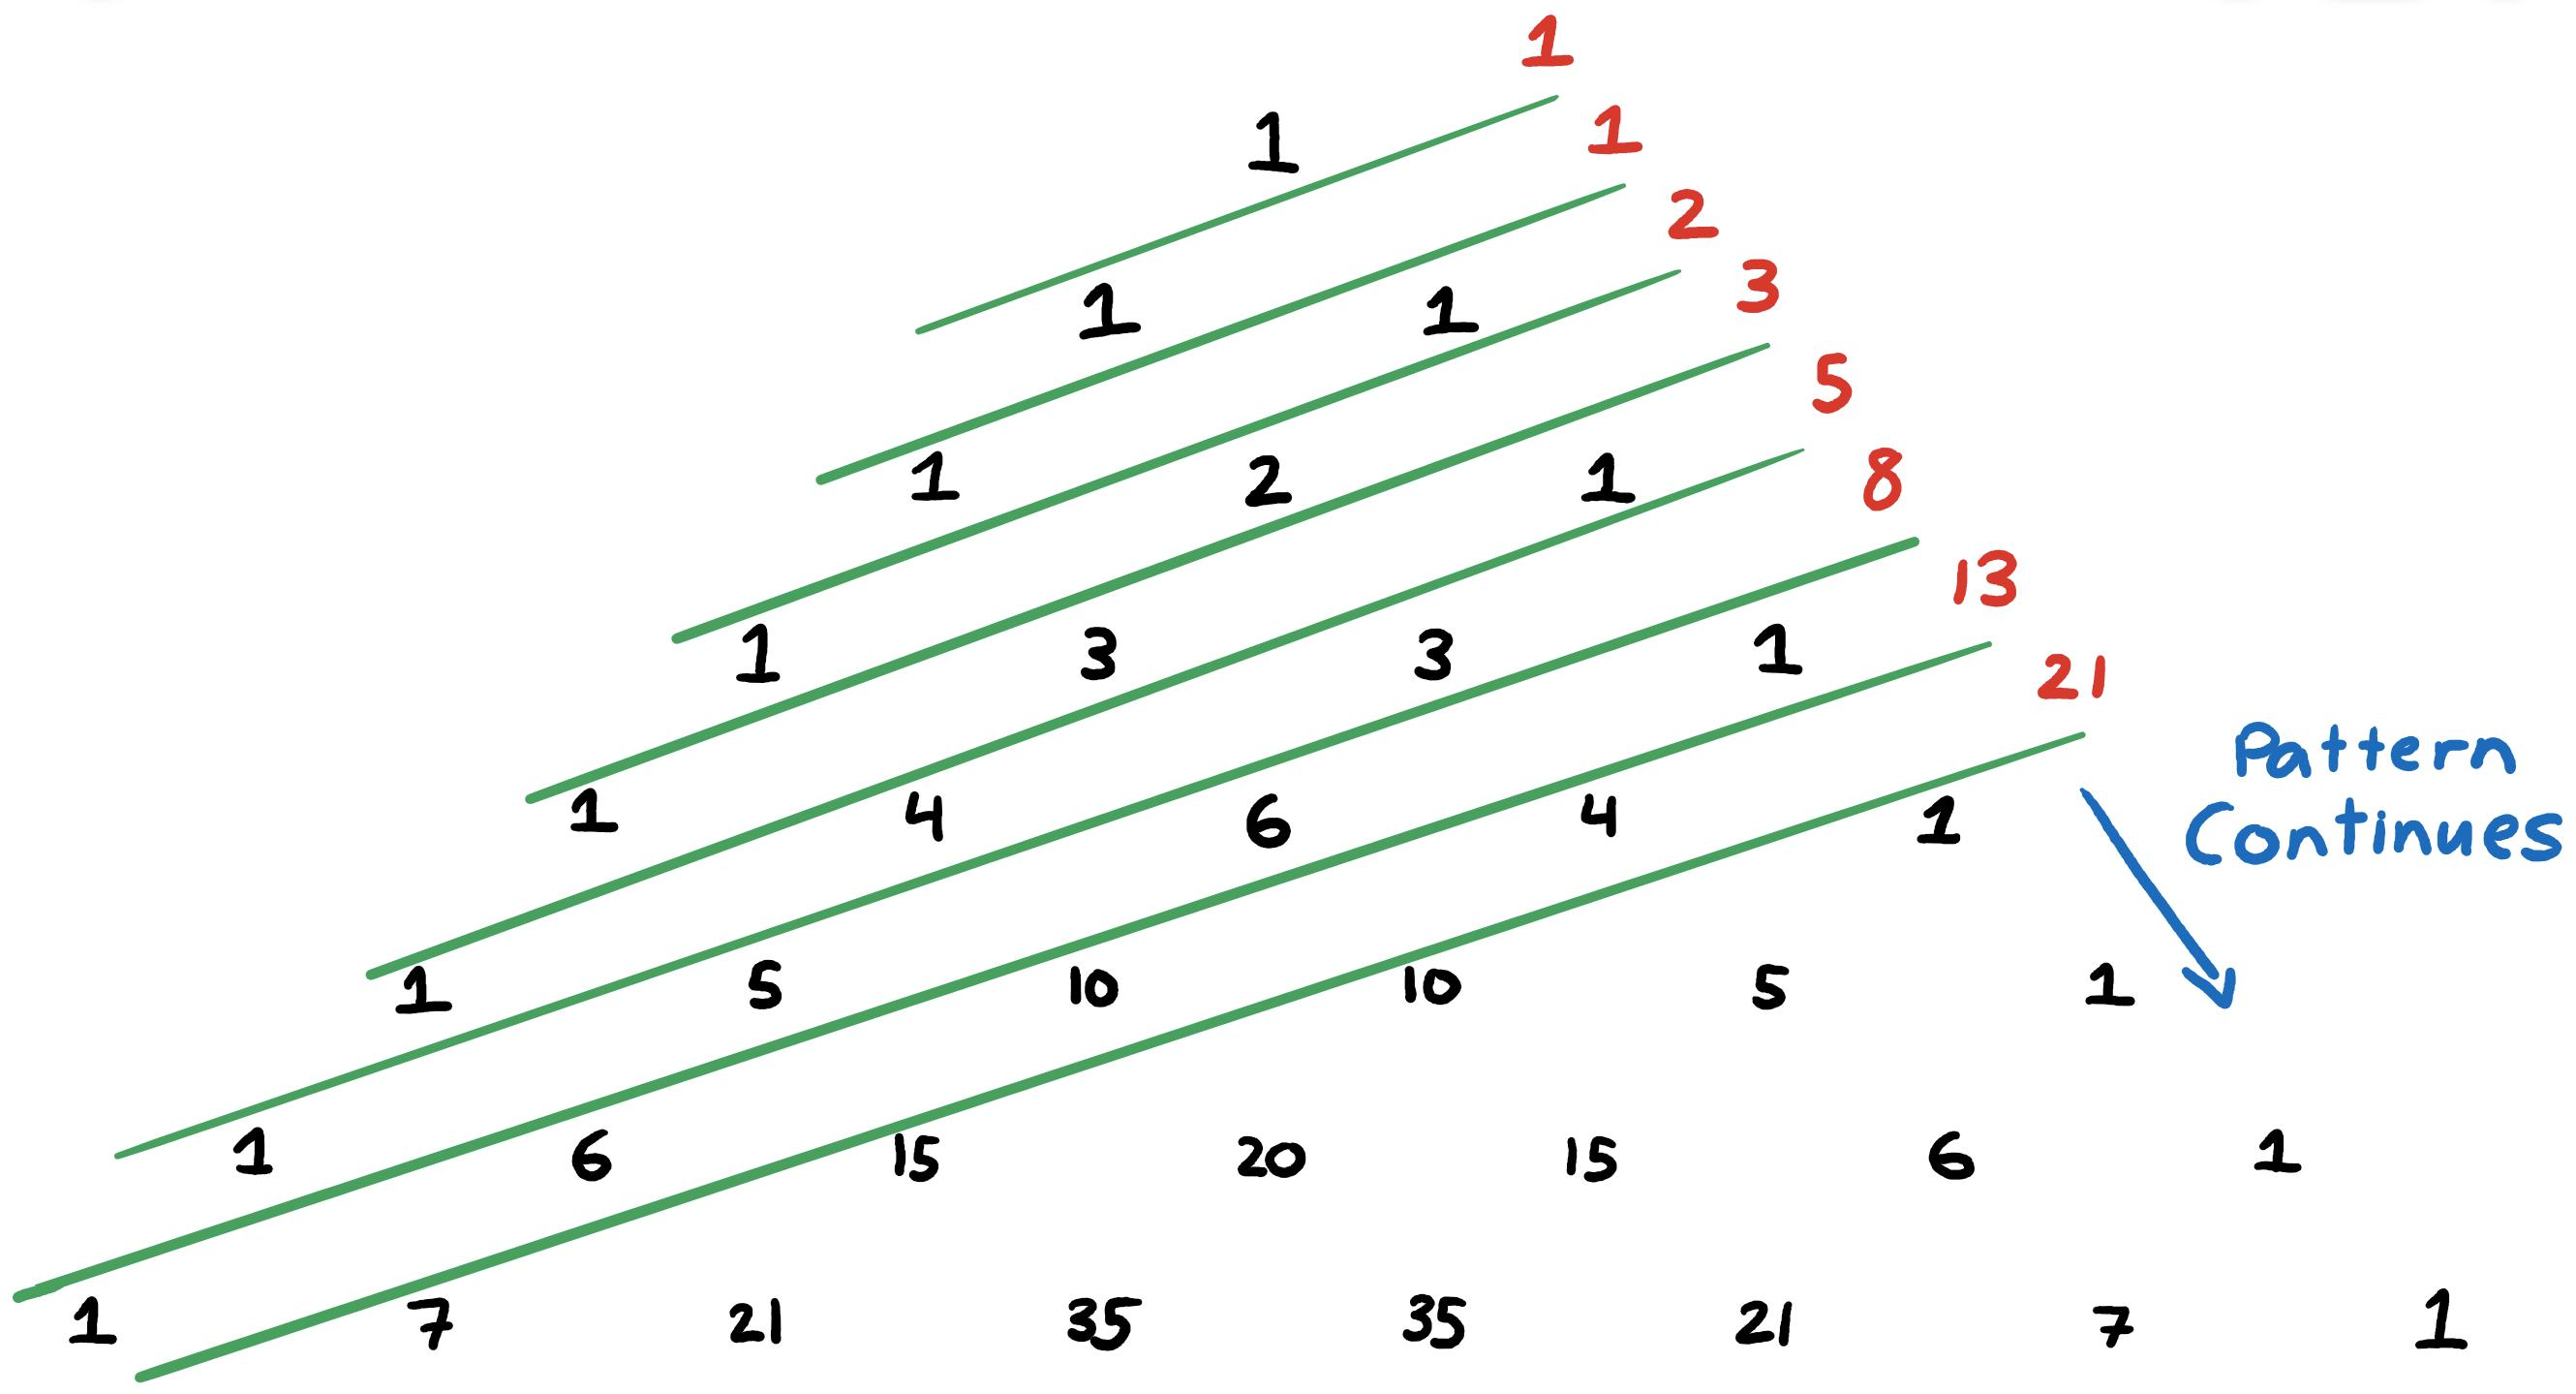
\includegraphics[width=0.6\textwidth]{pascalfibonacci}
\end{image}


\section{Fibonacci, Dominoes and Chess Boards}
We now investigate a counting problem that involves covering a chess board with dominoes. 
A normal chess board is $8 \times 8$ with $64$ squares.  
Our chess boards will be $2 \times n$ with $2n$ squares.  
A domino will cover two squares on our board and the question is: how many ways are there to cover our board with $n$ dominoes?
If $n=1$, the answer is obviously $1$.  If $n=2$ we see from the figure below that the answer is $2$.

\begin{image}
\begin{tikzpicture}
\draw (0,0) rectangle (2,1);
\draw (0,1) rectangle (2,2);
\node at (2.5,1) {and};
\draw (3,0) rectangle (4,2);
\draw (4,0) rectangle (5,2);
\node at (2.5,-0.5) {Covering a $2\times 2$ chess board with dominoes};
\end{tikzpicture}
\end{image}

For $n=3$, there are 3 possibilities as shown below:


\begin{image}
\begin{tikzpicture}[scale = 0.7]
\draw (0,0) rectangle (1,2);
\draw (1,0) rectangle (3,1);
\draw (1,1) rectangle (3,2);
%\node at (3.5,1) {and};

\draw (4,0) rectangle (5,2);
\draw (5,0) rectangle (6,2);
\draw (6,0) rectangle (7,2);
%\node at (7.5,1) {and};
\draw (8,0) rectangle (10,1);
\draw (8,1) rectangle (10,2);
\draw  (10,0) rectangle (11,2);
\node at (5.5,-0.5) {Covering a $2\times 3$ chess board with dominoes};
\end{tikzpicture}
\end{image}

\begin{proposition}
The number of ways to cover a $\, 2 \times n$ chess board with $n$ dominoes is the $(n+1)^{st}$ Fibonacci number, $f_{n+1}$.
\end{proposition}

\begin{proof}
We use strong induction. Suppose that the number of ways to cover a $2 \times n$ board is $f_{n+1}$ and that the number of ways to cover a 
$2 \times (n+1)$ board is $f_{n+2}$. We have seen that this is true for $n = 1$, establishing our base cases.
We now need to show that the number of coverings of a $2 \times (n+2)$ board is $f_{n+3}$. We partition the coverings into two groups.\\
Group 1) The domino that covers the upper left hand square is vertical.  The number of coverings of 
the $2 \times (n+2)$ board belonging to this group is simply the number of coverings of the $2 \times (n+1)$ board that 
lies to the right of this vertical tile.  By our inductive hypotheses, this is $f_{n+2}$.\\
Group 2) The domino that covers the upper left hand square is horizontal. This means that the domino below is also horizontal. 
The remaining part of the board that is not yet covered is $2 \times n$ and by the inductive hypotheses, 
the number of ways to complete the covering is $f_{n+1}$.\\
Since every covering belongs to either group 1 or group 2 and these two groups do not have any coverings in 
common (i.e. they form a partition of the set of all coverings), the number of coverings of a $2 \times (n+2)$ board 
is $f_{n+2} + f_{n+1}$ which equals $f_{n+3}$ by the recursive definition of the Fibonacci sequence.

\end{proof}

\begin{problem}(problem 4) Show that the number of ways to cover a $1 \times n$ chess board with dominoes and monominoes is also $f_{n+1}$.
\begin{hint}
A monomino is a $1 \times 1$ square
\end{hint}
\begin{hint}
Consider the first row of a covering of a $2 \times n$ board by dominoes
\end{hint}
\end{problem}
\end{document}




















